\chapter{Campaign Classes}\label{campaignclasses}


\pagecolor{gray}\afterpage{\nopagecolor}
\newpage
blah blah blah
\pagecolor{gray}\afterpage{\nopagecolor}
\fontfamily{pzc}
\selectfont

\newpage
\normalfont
%changing the page design temporarily
\changepage{9cm}{9.4cm}{-4.7cm}{-4.7cm}{}{-4.5cm}{}{}{}
%\noindent\rule{\textwidth}{\textheight}
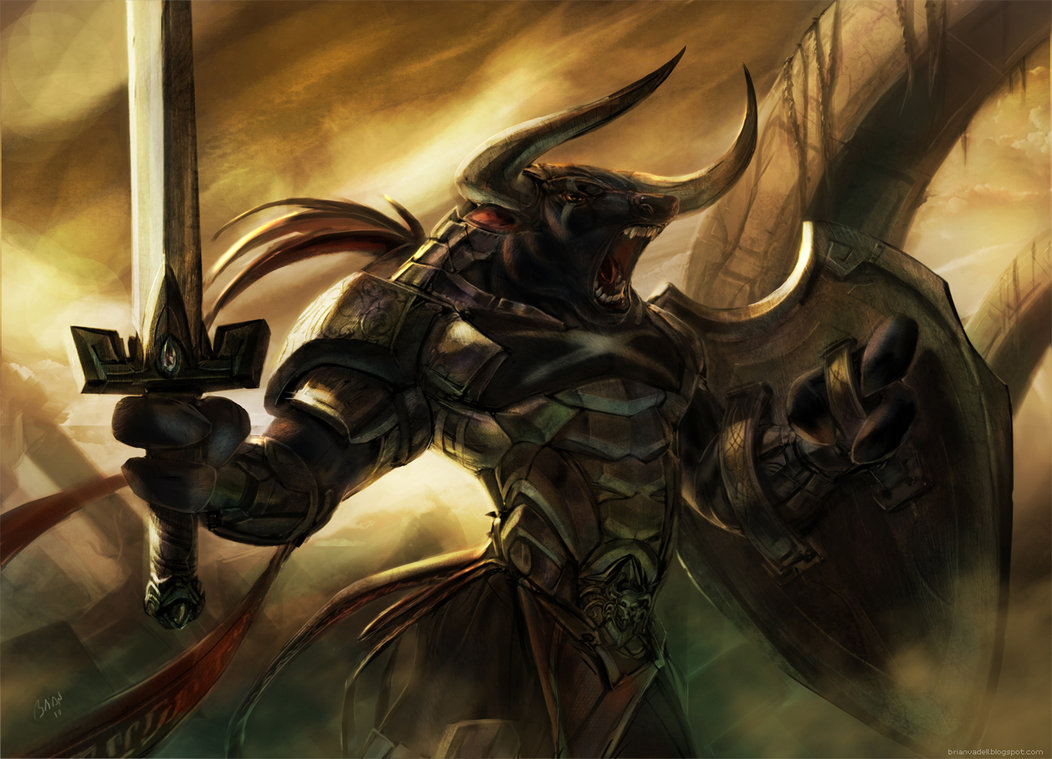
\includegraphics[width=\textwidth,height=\textheight]{minotaur_by_brianvadell}
\newpage

%restoring the standard settings
\changepage{-9cm}{-9.4cm}{4.7cm}{4.7cm}{}{4.5cm}{}{}{}
	These are special classes that build upon the existing core classes in the game. They reflect the influence that the setting has upon the character's own skills and talents. 
	There are essentially two types of Campaign Classes. Those that are tied to some regional background, and those tied to some faction. 
	Each faction provides some campaign classes, which maybe unlocked once they have joined and proved themselves within said faction. 
	Some campaign classes are also limited by what races may enter into it. 
\section{Dying Rat Minotaur} This faction campaign class is dedicated to maximising the lethality of his horns goring into someone on the charge. 

\section{Crusader Minotaur} 

% minotaur_by_brianvadell
%\begin{figure}[h]
%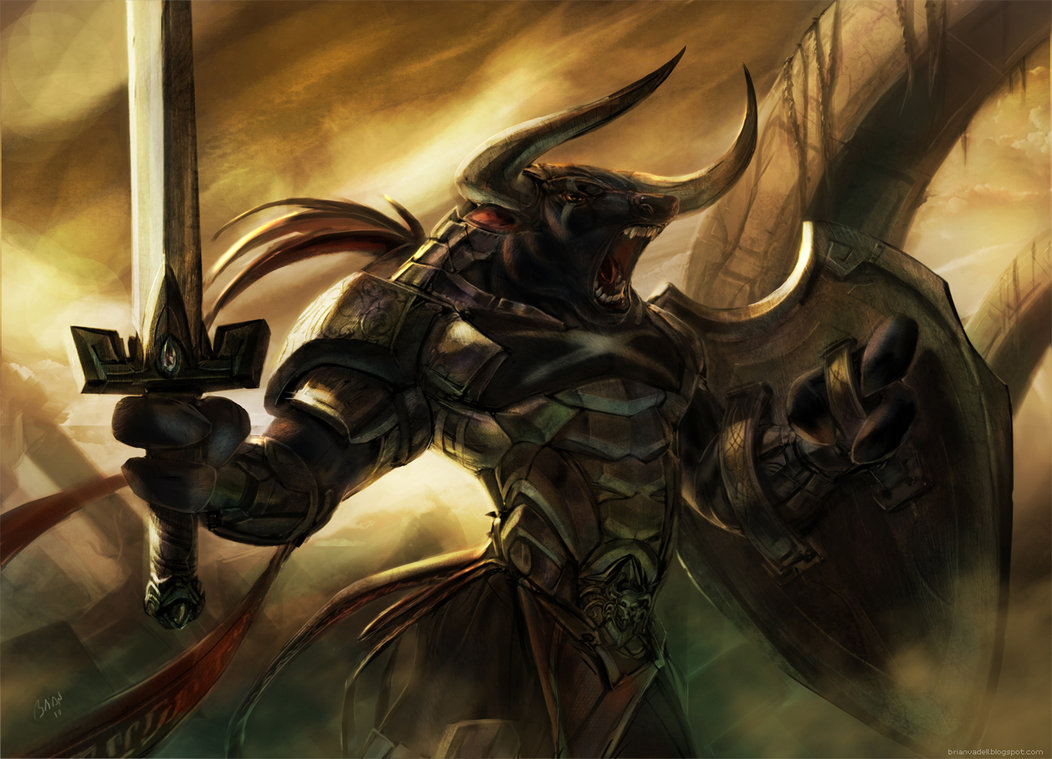
\includegraphics[width=\columnwidth]{minotaur_by_brianvadell}
%\end{figure}

\section{Midgaardian Spymaster} 
\section{Midgaardian Crusader}
\section{Midgaardian Knight Errant}
\section{Brouliard Cavalier}
\section{Brouliard Courtier}
\section{Brouliard Musketeer}
\section{Nessian Vikingr} This is an unusual class in that it is a combination of raider, trader and farmer. This is a hybrid class that aims to capture the realities and vicious myths of the vikingr people. 
\section{Nessian Ranger of the Black Thumb}
\section{Abloni Gladiator} A fearless warrior who is a master of melee combat (to the exclusion of other forms of combat). Uses a theatrical style of fighting that makes it very hard to use in massed formations (balancing aspect).
\section{Abloni Legionnaire Mercenary} A phalanx fighter whom is also a skilled manual labouring engineer (skilled in building quick fortifications, walls, roads, watch towers).
\section{Abyssian Witch Doctor} Known to the people of the Old Empire as a Witch Doctor, in fact the opposite is the case. The people of Abyssimiar have a more advanced understanding of medicine than than their ex-imperial cousins. From the perspective of the peasant however they are mystical and esoteric healers. 
\section{Abyssian Chariot Archer} 
A master of bow, spear and throwing axe. They are excellent at riding a Chariot. The class comes with a Loyal Henchmen whom fights with them. In exchange for the lack of normal henchmen, the class comes with other benefits.
\section{Venturer}
